\section{Evaluation}\label{sec:results}
In diesem Abschnitt werden die Ergebnisse des Experiments vorgestellt.
Dafür wird zunächst das Interview im Zusammenhang mit der Navigation durch die beiden Prototypen beschrieben.
Um einzelne Aussagen von den Teilnehmenden des Experiments zu belegen, werden Aussagen mit der Notation [P$x$, $y$] versehen.
Hierbei steht $x$ für die Nummer der Testperson und $y$ für die Zeile der Aussage im transkribierten Interviewprotokoll.
Im Anschluss werden die Auswertungen der Fragebögen vorgestellt.

\subsection{Allgemein}
% Verhalten Recherche
Zunächst werden Ergebnisse, welche sich auf allgemeine Faktoren beziehen, vorgestellt.
Dabei lässt sich festhalten, dass Personen bei ihrem Rechercheverhalten oder der Navigation unterschiedliche Ansprüche und Vorgehensweisen besitzen.
Person 1 beschreibt dabei sehr konkret ihre Vorgehensweise [P1, 28-44].
Zunächst recherchiert diese Person allgemein über ein Thema.
Anschließend werden speziellere Informationen gesucht, welche sich auf das Thema beziehen.
Zuletzt werden Themen, welche indirekt mit dem Thema in Verbindung stehen, recherchiert.
Andere Person tendieren dazu sich Artikel anzusehen, welche einen Bezug zum vorherigen Artikel haben [P3, 116-119; P6, 102-106].
Dabei scheinen diese Personen immer zwei Artikel bezüglich eines Themas zu lesen.
Person 6 begründet dies damit, dass ein Artikel meistens nicht genügt, um ein bestimmtes Thema zu verstehen.\\

%%% Fokus Titel
Durch den Aufbau des Experiments wurde ein verstärkter Fokus der Testpersonen auf die Überschriften der Artikel erzeugt.
Dies spiegelt sich bei sämtlichen Testpersonen darin wider, dass diese die Überschrift in den Vordergrund stellen.
Obwohl dies auf der einen Seite ein realistisches Verhalten abbildet, weil Testpersonen ihrem Interesse folgen, kann dies auf der anderen Seite zu einer Verzerrung der Ergebnisse führen.
Das liegt daran, dass der Fokus auf die Überschriften den Fokus auf die Titel der Artikel verlagert und nicht mehr auf die Navigation.
Vermehrt waren finanzielle oder aktuelle Themen für die Testpersonen interessant.
Person 2 erläutert zusätzlich, dass die Preissteigung von Diesel sie nicht betrifft, da sie keinen Diesel fährt [P2, 54-67].\\

% Clickbait & Werbung
Allgemein wurde das Thema Clickbait von einigen Testpersonen angesprochen [P2, 228-230; P4, 107; P4, 155-158; P5, 5-6; P10, 46-47].
Dieses Thema hat nicht direkt, sondern indirekt, etwas mit der Navigation durch die Prototypen zu tun.
Person 5 macht deutlich, dass sie diese Artikel aus Prinzip nicht klicken würde, wenn es sich um reißerische Überschriften handelt [P5, 5-6].
Person 10 hingegen erwähnt zwar, dass diese Artikel \glqq nichts aussagen\grqq{}, würde diese jedoch trotzdem lesen [P10, 46-47].
Hier wird ebenfalls deutlich, dass die Gruppe von Nutzenden keineswegs homogen ist.
Auch der Aspekt von Werbung in Artikeln wurde von diesen beiden Testpersonen angesprochen [P5, 3-4; P10, 19-21].
Das Problem Clickbait wurde bereits näher in \autoref{subsec:challenges} beschrieben.
Da die Artikel in beiden Prototypen von einer Quelle stammt, welche Klicks von Nutzenden maximieren möchten, spiegelt sich auch der Aspekt von Clickbait in den Artikeln wider.
Werbungen werden aus finanziellen Gründen in Artikeln platziert.
Sie sind einer der Gründe, weswegen die Klicks von Nutzenden als Metrik verwendet werden.

\subsection{Liste}
Während der Navigation durch die Liste ist bei den Testpersonen aufgefallen, dass sie Liste nicht intuitiv als Sortierung nach Ähnlichkeit interpretiert haben.
Auch in diesem Fall sind die Teilnehmenden nach Überschriften von Artikeln vorgegangen, um bei den Aufgaben ähnliche oder unähnliche Artikel zu finden [P2, 250-254].
Dies könnte auf unterschiedliche Arten interpretiert werden.
Zum einen könnte es daran liegen, dass das Experiment keinen ausreichenden Bezug auf andere Listensysteme mit \acp{RS} hat.
Zum anderen könnte es daran liegen, dass die Testpersonen kein allgemeines Verständnis von Listen, welche durch content-based \acp{RS} erstellt werden, haben.
Ebenfalls wurden in zwei Fällen unbekannte Überschriften als unähnlich zu einem vorgegebenen Artikel interpretiert [P3, 68-72; P4, 133-141].\\

% Position Bias
Die in \autoref{subsec:challenges} erwähnte Problematik, dass Listen eine Art von Position Bias mit sich bringen, konnte durch eine Aussage bestätigt werden [P1, 48-53].
Person 1 erwähnte explizit, dass sie die Liste von oben nach unten liest und auch in dieser Reihenfolge konsumiert.
Eine weitere interessante Beobachtung brachte die Reihenfolge in der Personen mit den Prototypen interagieren hervor.
Die erste Aussage von Person 2 war, nachdem sie durch den Begriffsverband navigiert hatte, dass die Liste \glqq relativ zusammenhangslos\grqq{} sei und dass sie keine Form der Kategorisierung erkennt [P2, 202-203].
Sie machte zusätzlich beim Beantworten vom Fragebogen \ac{QUESI}, dass ihr diese Form der Kategorisierung in der Liste gefehlt hat [P2, 262-265].
Im gleichen Satz wurde jedoch auch erwähnt, dass Listen sehr einfach zu verwenden sind.
Dieser Gedanke wird von mehreren Testpersonen geteilt und auch von Person 3 zusammengefasst [P3, 74-78].
Listen sind für die Testpersonen einfach zugänglich und weisen eine geringere Komplexität als ein Begriffsverband auf.\\

% Umdenken 
Die einzigen beiden Personen, welche erwähnten, dass sie nur die Liste privat verwenden würden, waren Person 1 und Person 3.
Person 1 begründet dies damit, dass die Navigation durch den Begriffsverband zu umständlich ist [P1, 388-401].
Die Kategorisierung wird zwar als positiv empfunden, aber die Darstellungsform ist zu unübersichtlich.
Sie erwähnt explizit, dass der Gedanke nicht fallen muss: \glqq In welche Kategorie will ich mich denn jetzt begeben?\grqq{}.
In diesem Fall lässt sich jedoch auch sagen, dass das Experiment auf den ersten Blick erfolgreich war, da bei den Testpersonen ein Umdenken stattgefunden hat.
Schließlich war das Ziel des Experiments, dass Personen sich zuerst Gedanken über die Kategorie machen und sich im Anschluss Artikel aus dieser Kategorie aussuchen.
Dieses müsste jedoch noch weiter verfolgt werden, um eine konkretere Aussage treffen zu können.
Schließlich ist damit noch nicht bewiesen, dass dies auch eine Auseinandersetzung mit kritischeren Inhalten fördert.\\

% Liste simpel
Auch Person 3 erwähnt, dass Listen einfacher zu bedienen sind [P3, 178-184].
Sie möchte vermeiden über die Navigation nachzudenken und stattdessen Optionen präsentiert zu bekommen, welche auf ihre Interessen zugeschnitten sind.
Auch Person 3 erwähnt, dass explizit, dass sie kein Interesse daran hat, sich Gedanken über die Kategorisierung zu machen [P3, 212-214].
Der Grund hierfür liegt darin, dass die Navigation durch die verschiedenen Kategorien zu viel Zeit in Anspruch nehmen würde.
Person 3 bevorzugt es, Inhalte in kurzen Zeitintervallen zu konsumieren, was dazu führt, dass sie weniger Zeit für das Navigieren aufwenden möchte.
In diesem Fall ist eine Listendarstellung dem Begriffsverband vorzuziehen, da die Navigation durch auf Personen zugeschnittene Artikel einen geringeren Zeitaufwand mit sich bringt als das eigenständige Suchen von Artikeln.

\subsection{Begriffsverband}
Das Tutorial wies einige Probleme auf.
Dies konnte, unter anderem, durch die Aufgaben im Tutorial gezeigt werden.
Alle Testpersonen konnten die Anzahl der Gegenstände in der Kategorie pflanzliche Nahrungsmittel korrekt bestimmen.
Jedoch wurde die Gesamtanzahl der Gegenstände bei der Kategorie Nahrungsmittel bei vier Personen falsch beantwortet.
Das Problem daran ist, dass die Testpersonen die Anzahl der Gegenstände in der Kategorie pflanzliche Nahrungsmitteln mit den Gegenständen der Kategorie tierische Nahrungsmittel aufsummiert haben [P2, 17-20; P4, 16-17].
Auf diese Weise wurde jedoch der Gegenstand Rindfleischburger doppelt gezählt.
Zwei der Personen haben zusätzlich zu den genannten Kategorien den Rindfleischburger mit in die Kategorie Nahrungsmittel aufgenommen [P3, 81-85; P5, 7-10].
Auf diese Art und Weise wurde der Rindfleischburger dreifach gezählt.
Dies deutet darauf hin, dass im Tutorial ein Knoten mit implizit gegebenen Merkmalen nicht ausreichend erklärt wurde.
Ebenfalls müsste deutlich gemacht werden, dass Rechenoperationen wie die Addition der Anzahl von zwei Knoten nicht immer möglich sind.
In einem zukünftigen Tutorial könnte es sinnvoll sein die einzelnen Gegenstände aufzuzählen, anstatt die Gesamtanzahl zu bestimmen.
Dies würde das Verständnis der Darstellung im Begriffsverband besser stärker.
Zusätzlich wird die Kompetenz vom Bestimmen einer konkreten Anzahl Testpersonen im Endprodukt nicht benötigt.\\

% Rindfleischburger 
Im Tutorial ist allgemein aufgefallen, dass der Rindfleischburger für die Testpersonen verwirrend war.
Dieser wurde zwar analog zum vorherigem Beispiel mit dem Gegenstand Schwein in \autoref{fig:begriffsverband-tiere} dargestellt, jedoch wurden im Zusammenhang vermutlich zu viele Konzepte gleichzeitig erklärt.
Dies führte dazu, dass in diesem Fall das im Interview eine aktive Erklärung zu diesem Knoten notwendig war.
Dabei wurde die Zusammensetzung eines Rindfleischburgers und die Kategorisierung in tierische und pflanzliche Nahrungsmittel erläutert.
Das aktive Eingreifen ist notwendig gewesen, da ansonsten die Darstellung von Artikeln im Begriffsverband nicht verstanden worden wäre.\\

% Letzte Seite im Tutorial
Für die Teilnehmenden des Experiments war jedoch eindeutig die letzte Seite des Tutorials schwierig.
Diese beinhaltete die Liste, welche nach Anzahl der Welten sortiert war.
Es kamen bei allen Personen, bis auf Person 5 und Person 10, auf, dass diese Seite eine zu hohe Komplexität aufweist.
Vermutlich hat die Erklärung und das von Person 2 erwähnte Problem dazu beigetragen, dass diese Seite als sehr komplex empfunden wurde.
Person 2 erwähnte, dass der zusätzliche Knoten für Verwirrung gesorgt hat [P2, 29-41].
In diesem Fall wäre eine Verbesserung, dass der Knoten mit dem Merkmal Staat nicht aufgetrennt werden sollte.
Dies ist ein Problem, da die Testpersonen die Kompetenz von aufgetrennten Knoten im Tutorial nicht erworben haben.
Stattdessen sollte Schritt für Schritt erklärt werden, wie die Liste sich zusammensetzt.\\

% Zahlenbeispiel
Person 1 erwähnte einen weiteren Verbesserungsvorschlag für das Tutorial.
Sie erwähnte, dass es hilfreich wäre, wenn im gegebenen Beispiel die Anzahl der Gegenstände als Zahl doppelt vorkommen sollen [P1, 123-138].
Der Grund dafür ist, dass es ansonsten zu Fehlinterpretationen kommen kann, da Personen von einer aufsteigenden Nummerierung ausgehen.
Dieses Problem ist, bis auf die kurzzeitige Verwirrung von Person 1, nicht aufgetreten.
Jedoch ist es sinnvoll jegliche Verwirrung zu vermeiden, da dies die Kompetenzen der Testpersonen beeinträchtigen kann.
Ein verwirrendes Tutorial kann dazu führen, dass der Lernerfolg oder die Motivation negativ beeinflusst wird.
Aus diesem Grund sollten jegliche Risiken minimiert werden. \\

% Tutorial = Gut
Trotz einiger Kritikpunkte und Komplikationen wurde das Tutorial als hilfreich empfunden.
Person 2 äußert sich positiv über das Tutorial und ist der Meinung, dass das Tutorial den strukturellen Zusammenhang im Begriffsverband deutlich macht [P2, 182-189].
Ohne das Tutorial müsste sie über Trial-and-Error durch den Begriffsverband navigieren, ohne zu wissen, wie Zusammenhänge im Begriffsverband funktionieren.
Auch an einer anderen Stelle hat das Tutorial eine positive Wirkung.
Zwei Personen nehmen bei der Navigation durch den Begriffsverband zum Tutorial Bezug [P1, 204-205; P3, 99-102].
Dies zeigt, dass Kompetenzen aus dem Tutorial erfolgreich auf die Navigation im Begriffsverband übertragen werden konnten.\\

% Unklare Begriffe
Im Tutorial und auch im Prototyp gibt es ebenfalls Begriffe, welche unklar sind oder für Verwirrung sorgen.
Der Begriff Knoten zum Beispiel ist für Person 6 unklar [P6, 3].
Dieser Begriff sollte im Tutorial zusätzlich erklärt werden, um Personen die Möglichkeit zu geben, sich mit dem Begriff vertraut zu machen.
Zusätzlich sorgt die Benennung der Welt Grün aus den \ac{EC} für mehrdeutige Interpretationen [P4, 50-52].
Grün könnte ebenfalls als die politische Partei der Grünen interpretiert werden.
Da die Begriffe nicht zwangsläufig mit den Begriffen der \ac{EC} übereinstimmen müssen, könnte stattdessen der Begriff Umwelt verwendet werden.
Dies gilt auch für die nicht notwendige Einführung des Begriffs Welt [P1, 171-173].
Dieser Begriff ist nicht notwendig, da Welt im Begriffsverband gleichzusetzen ist mit dem Begriff Kategorie.\\

% Prototyp interessant
Abseits vom Tutorial wird der zugehörige Prototyp als interessant empfunden [P1, 101; P6, 143-148].
Obwohl Testperson 3 die Darstellung als Liste präferiert, ist sie der Meinung, dass die Kategorisierung von Inhalten sinnvoll ist [P3, 190-195].
Ebenfalls wird betont, dass Zusammenhänge im Begriffsverband deutlich werden.
Die Zusammenhänge sollen laut Person 9 im Vergleich zur Liste übersichtlicher sein [P9, 149-150].
Diese Person ist ebenfalls der Meinung, dass die Kategorisierung hilfreich ist, um Zusammenhänge zu verstehen [P9, 105-107].
Sie benennt die Kategorisierung als hilfreich, um zu verstehen, mit welcher Intention ein Artikel geschrieben wurde.
Dieser Gedanke zeigt, dass die Darstellungsform im Begriffsverband die Filterblase für Nutzende des Systems sichtbar macht.
Person 4 illustriert eine weitere positive Eigenschaft der Kategorisierung [P4, 198-203].
Sie erwähnt, dass die Kategorisierung hilfreicher für ein Verständnis ist als nur ein Titel.
Diese Eigenschaft der Kategorisierung fasst laut Person auch auf positive Art und Weise Inhalte zusammen [P5, 134-142].\\

% Artikelansicht intressant
Auch die Artikelansicht im Begriffsverband wird als positiv empfunden [P8, 20-22].
Speziell fehlt jedoch die Möglichkeit, wie im Tutorial, hervorgehobene Textsegmente zu sehen, welche die Kategorisierung von Artikeln in die unterschiedlichen Welten der \ac{EC} verdeutlichen [P3, 99-102; P5, 112-126].
Eine permanente Hervorhebung der Textsegmente könnte den Lesefluss stören.
Aus diesem Grund wäre es sinnvoll, dass die Textsegmente nur bei Bedarf hervorgehoben werden können.
Dies könnte durch einen Toggle-Button realisiert werden.
Person 10 macht darauf aufmerksam, dass es durch die Hervorhebung von Kategorien auch einfacher möglich sein könnte negative Kommentare zu verfassen [P10, 32-36].
Insbesondere, wenn dieses Problem aus politischer Sicht betrachtet wird, könnte es sehr wahrscheinlich sein, dass negative Kommentare bei der gegenüberliegenden politischen Richtung verfasst werden.
Diese Herausforderung sollte bei der Weiterentwicklung des Prototyps berücksichtigt werden.\\

% Farben
Die farbliche Repräsentation von Rechtfertigungen wird von den Teilnehmenden des Experiments als sinnvoll empfunden [P2, 27-28].
Sie ermöglichen und unterstützen unter anderem das Rechercheverhalten von Person 1 [P1, 270-294]. % auch erwähnt, dass es unklar ist
Diese Person präferiert ist sich zunächst positive Rechtfertigungen und im zweiten Schritt negative Rechtfertigungen anzusehen.
Mithilfe dieses Verhaltens kann die Person sich ein Gesamtbild über ein gegebenes Thema machen.
Auch in diesem Fall trägt die Darstellungsform dazu bei, dass die Rechtfertigungen der Artikel deutlich sichtbar werden [P2, 301-307].
Die anteilmäßige Darstellung wird von Person 5 als intuitiv verstanden [P5, 156-160].
Person 6 erweitert diese Aussage und erklärt, dass diese Darstellungsform praktisch und übersichtlich ist [P6, 157-159].
Diese Aussagen deuten darauf hin, dass die Darstellung von Rechtfertigungen im Begriffsverband in der Masterarbeit weniger Probleme bereitet als in der Vorstudie.
Allerdings ist ein eindeutiger Vergleich zwischen der Darstellungsform der Vorstudie und der Masterarbeit erforderlich, um diese Aussage zu bestätigen. \\

% Viel positiv
Ein weiter Vorteil der farblichen Repräsentation ist es ein auf einem Blick ein Gesamtbild über die Rechtfertigungen aller Welten zu erhalten.
Es wird jedoch angemerkt, dass der gegebene Datensatz zu wenig negative Rechtfertigungen enthält [P4, 68-70; P5, 234-236].
Dies muss jedoch nicht zwangsläufig ein Problem sein, da Rechtfertigungen bei realen und größeren Datensätzen nicht zwangsläufig gleichmäßig verteilt sind.
Ein Problem ist jedoch, dass bei einer Interaktion mit der Kategorie die Artikel kein Indiz für die Rechtfertigung einer Welt erhalten.
Dies ist ein Problem, weil Nutzende des Systems nicht erkennen können, ob ein Artikel positiv, negativ oder aus beiden Rechtfertigungen besteht.
Eine Möglichkeit dieses Problem zu lösen wäre, dass die Artikel in der Kategorieansicht eine Farbe erhalten, welche die Rechtfertigung der Welt darstellt [P6, 52-60].
Dies ist jedoch nur möglich, wenn eine Kategorie angeklickt wird, welche nur eine Welt repräsentiert.
Bei Knoten, welche mehr als einer Welt repräsentieren, müssten mehrere Farben verwendet werden, was wiederum die Übersichtlichkeit beeinträchtigen könnte.\\

% Mehrere Merkmale
Bei Knoten mit mehreren Merkmalen gab es unterschiedliche Meinungen.
Person 2 äußerte, dass sie es für sinnvoller hält, wenn die impliziten Merkmale explizit ausgeschrieben werden [P2, 285-295].
Person 5 hingegen ist der Meinung, dass dies nicht notwendig ist und zu viel Text ablenken würde [P5, 176-178].
Diese Meinung bestätigt die in der Masterarbeit vorgeschlagene Lösung, möglichst wenig Text im Begriffsverband zu verwenden, um die Übersichtlichkeit zu erhalten.
Da der Vorschlag von Person 2 jedoch auch seine Berechtigung hat, wurde im Interview spontan eine Lösung für dieses Problem gefunden [P5, 179-182].
Dabei soll das Hovern über einem Knoten die impliziten Merkmale anzeigen.
Auf diese Art und Weise wird die Übersichtlichkeit erhalten und die Informationen sind trotzdem bei Bedarf verfügbar.
Person 5 äußerte eine weitere Meinung in Bezug auf die Merkmale von Knoten [P5, 147-153].
Sie ist der Meinung, dass beim grau färben von Knoten Merkmale weiterhin angezeigt werden sollten.
Der Grund dafür ist, dass Merkmale nicht mehr sichtbar sind und die Nutzenden in die vorherige Ansicht zurückkehren müssen, um sich das Merkmal zu merken.\\

% Liste und Artikelansicht
Bezüglich der Artikel- und Kategorieansicht wurden ebenfalls unterschiedliche Meinungen geäußert.
Meistens wurden beide Ansichten ausprobiert, aber die Kategorieansicht wurde präferiert.
Der Grund hierfür liegt daran, dass die Kategorieansicht für eine bessere Übersicht und weniger Klicks sorgt [P2, 92-100; P4, 71-76].
Die Übersicht wird als besser empfunden, da mehr Artikel als in der Artikelansicht aufgelistet werden.
Dies führt wiederum zu weniger Klicks, da die Nutzenden nicht unbedingt weitere Knoten anklicken müssen, um mehr Artikel einsehen zu können.
Das Problem bei der Kategorieansicht ist jedoch wiederum, dass ähnliche Herausforderungen wie bei einer Liste mit content-based \ac{RS} auftreten.
Bestätigt wird dieser Verdacht dadurch, dass Person 1 auch bei dieser Liste \glqq einfach den Ersten\grqq{} Artikel anklickt [P1, 261-269].\\

% Verständnis
Ähnlich wie bei der Darstellung von Artikeln als Liste gab es auch bei der Darstellung als Begriffsverband Verständnisprobleme.
Das Verständnis für die Funktionsweise des Begriffsverbandes wurde durch unterschiedlichen Aufgaben abgefragt.
Jedoch konnten nur Person 2 und Person 5 ähnliche und unähnliche Artikel anhand der Darstellung im Begriffsverband finden [P2, 162-177; P5, 197-208].
Alle anderen Personen versuchten die Artikel anhand der Überschriften zu unterscheiden.
Dies ist teils gelungen, jedoch wird dies nicht beachtet, da keine Erklärung anhand der Darstellung erfolgt ist.
Beide Personen, welche die Aufgabe erfolgreich gelöst haben, hatten im Informatikstudium mehrfach Kontakt mit Graphen.
Aus diesem Grund ist nicht auszuschließen, dass einige Kompetenzen, im Vergleich zu anderen Personen, auf den Begriffsverband übertragen wurden. \\

% Übergeordneter Knoten
Dies heißt jedoch nicht im Umkehrschluss, dass die anderen Teilnehmenden keine Kompetenzen im Umgang mit dem Begriffsverband besitzen.
Um Artikel im Begriffsverband zu finden, haben einige Testpersonen den obersten Knoten im Graphen verwendet, um alle Artikel aufzulisten [P1, 329-333; P3, 132-135; P4, 80-82; P10, 58].
Gerade diese Tatsache zeigt ein Verständnis der Testpersonen für den Umfang eines Begriffs.
Person 2 geht sogar einen Schritt weiter und benennt den obersten Knoten als Elektromobilität [P2, 43-45].
Dies ist ein interessanter Aspekt, da die Elektromobilität nur ein Thema von vielen unterschiedlichen Themen ist, welche mit einem Begriffsverband abgebildet werden können.
Das Experiment zeigt nur einen kleinen Ausschnitt aus allen möglichen Themen, welche journalistisch abgedeckt werden.
In einem Interview ist das Konzept des Teilverbandes gefallen [P4, 179-188].
Ein Teilverband ist eine Teilmenge eines Verbandes, welche selbst ein Verband ist.
In diesem Fall könnte Elektromobilität ein Teilverband von Mobilität sein, welches wiederum ein Verband von Verkehr sein könnte.
Dieses Konzept ist nicht Teil der Masterarbeit, aber könnte eine interessante Erweiterung des Begriffsverbandes für weitere Prototypen darstellen.

\subsection{AttrakDiff}
\begin{figure}[!ht]
    \centering
    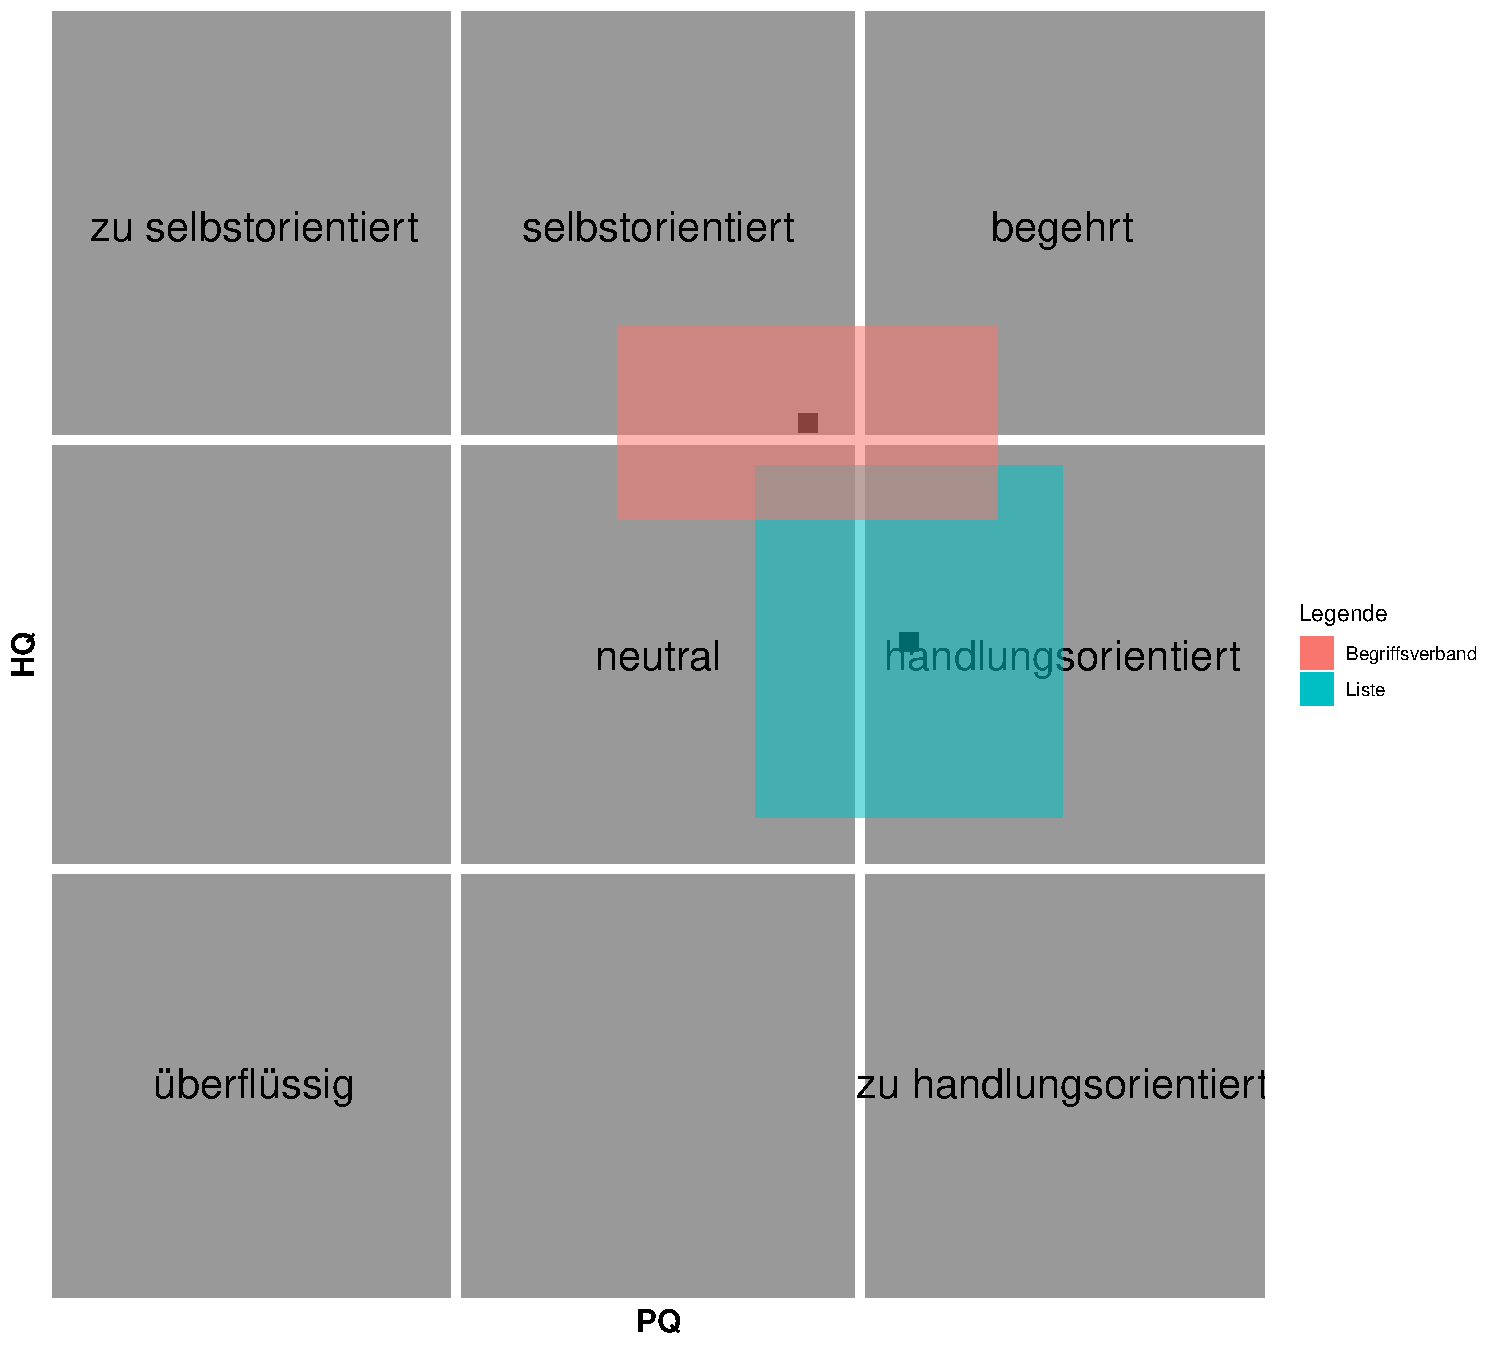
\includegraphics[width=0.7\columnwidth]{figures/attrakdiff-squares.pdf}
    \caption{\label{fig:attrakdiff-squares}AttrakDiff - Portfolio-Darstellung}
\end{figure}

\begin{figure}[!ht]
    \centering
    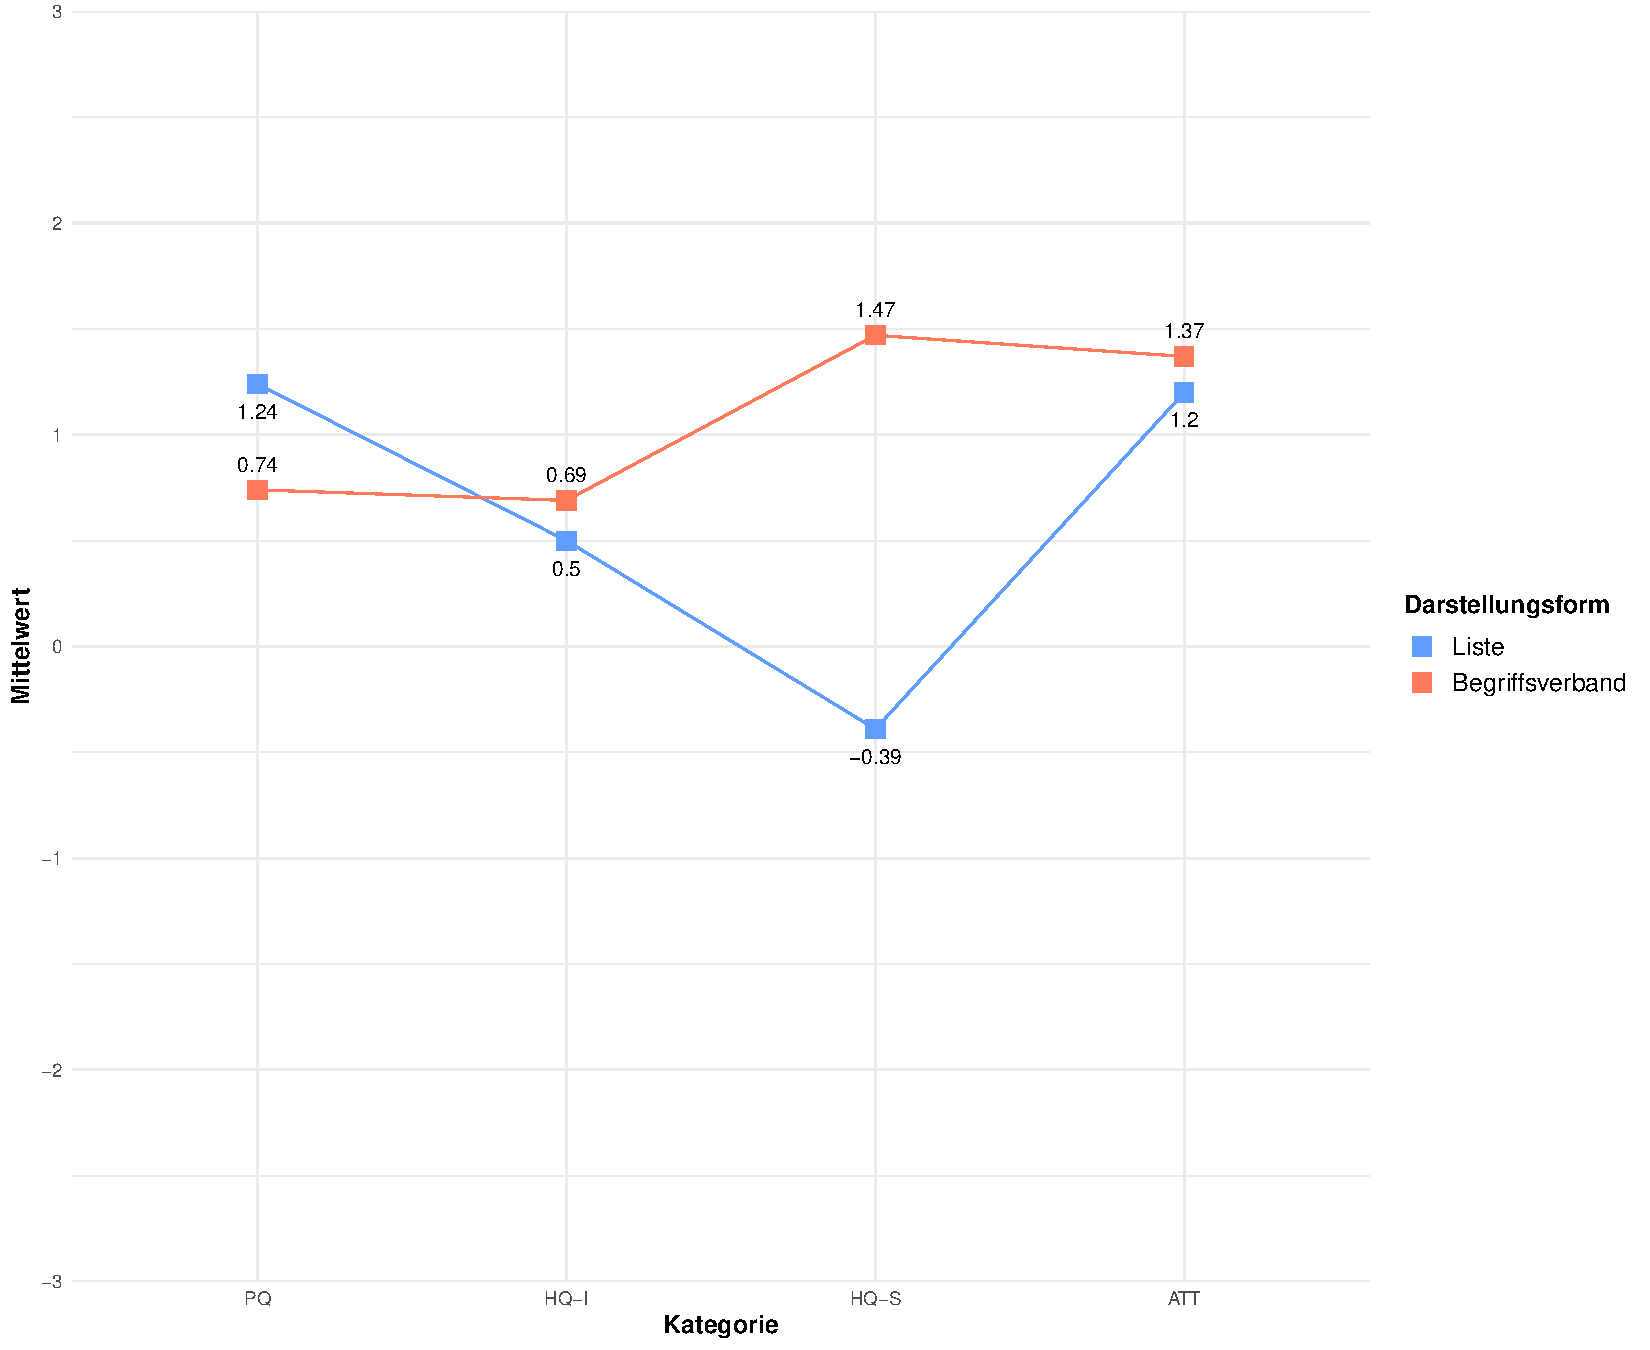
\includegraphics[width=0.7\columnwidth]{figures/attrakdiff-line.pdf}
    \caption{\label{fig:attrakdiff-line}AttrakDiff - Diagramm der Mittelwerte}
\end{figure}

\textcolor{red}{TODO}
\subsection{QUESI}
\begin{center}
    \begin{table}[!ht]
        \centering
        \begin{tabular}{|l|c|c|c|c|c|c|}
            \hline
                                                 & Arbeitsbelastung & Ziele & Lernen & Vertrautheit & Fehler & Gesamt \\ \hline \hline
            \multicolumn{1}{|c|}{$\overline{x}$} & 4,4              & 4,4   & 4,7    & 4,67         & 5      & 4,61   \\ \hline
            \multicolumn{1}{|c|}{SD}             & 0,93             & 0,81  & 0,79   & 0,66         & 0      & 0,77   \\ \hline
        \end{tabular}
        \caption{QUESI - Liste}
        \label{table:quesi-list}
    \end{table}
\end{center}

\begin{center}
    \begin{table}[!ht]
        \centering
        \begin{tabular}{|l|c|c|c|c|c|c|}
            \hline
                                                 & Arbeitsbelastung & Ziele & Lernen & Vertrautheit & Fehler & Gesamt \\ \hline \hline
            \multicolumn{1}{|c|}{$\overline{x}$} & 3,23             & 4,37  & 3,27   & 3,83         & 4,25   & 3,76   \\ \hline
            \multicolumn{1}{|c|}{SD}             & 1,41             & 0,76  & 1,39   & 1,29         & 0,85   & 1,27   \\ \hline
        \end{tabular}
        \caption{QUESI - Begriffsverband}
        \label{table:quesi-fca}
    \end{table}
\end{center}


\subsection{Eigener Fragebogen}
%%% YouTube News 
% P1, 373-375

%%% Kategorisierung wird als gut empfunden, aber Liste bevorzugt
% P1, 390-392
% P5, 227-228 -> Bequemlichkeit

%%% pref. Recommendersystem
% P5, 76-78 -> bewusste Entscheidung für Kategorie
% P5, 85-88 -> Aktive Suche = Google + nicht entscheidungsfreudig

%%% Bei Liste fehlt Zusammenhang 
% P5, 241-244

%%% Filter für Graph
% P6, 147-148

%%% Einarbeitungszeit für Graph
% P7, 127-130
